\chapter{Desarrollo} \label{development}
En este capítulo se describe la aplicación web eFuel con sus módulos y funcionalidades, luego se narra cómo fue el desarrollo del proyecto. El desarrollo se divide en 3 fases: una fase de inducción donde el pasante se familiarizó con las herramientas y tecnologías necesarias para realizar el proyecto, una fase de desarrollo que consta de 6 Iteraciones de Scrum y una última fase de documentación.

A continuación la descripción de la aplicación seguido de las fases del desarrollo de la misma durante el proyecto de pasantía.

\section{La aplicación web eFuel}
\subsection{Versión original de eFuel}
Una primera versión de eFuel fue desarrollada por la empresa anteriormente y estaba  conformada por 4 módulos básicos:

\begin{itemize}
    \item \emph{Seguridad}: controlaba el acceso a laaplicación y sus datos.
    \item \emph{Pedidos}: inserción de pedidos de combustible.
    \item \emph{Pagos}: operaba como auxiliar contable del sistema de facturación interno de la organización (mayorista). 
    \item \emph{Datos}: ofrecía la posibilidad de activar y desactivar registros correspondientes a clientes, productos y otros parámetros no disponibles en el ERP de la organización. Adicionalmente poseía una bitácora que registraba las operaciones realizadas en el sistema.
\end{itemize}

Esta versión fue desarrollada hace más de 10 años utilizando Classic ASP, un motor de scripting para servidores cuya última versión fue desarrollada en el año 2000. Classic ASP fue reemplazada por ASP.NET en el año 2002, por esta razón no se pudo replicar la instalación de esta versión.

Para este proyecto se desea desarrollar una versión de la aplicación web eFuel basada en tecnologías modernas como ASP.NET y Umbraco. Se usaron documentos de la versión original para guiar el desarrollo de la nueva versión de eFuel, especialmente en el diseño de las entidades de la base datos y en las funcionalidades generales (módulos) del sistema.

\subsection{Nueva versión de eFuel}
La nueva versión de eFuel desarrollada para este proyecto es una aplicación web que permite a las estaciones de servicio de combustible la colocación de sus pedidos al mayorista. La aplicación permite consultar información del estado de los pedidos (si fueron despachados y si fueron pagados), asociar facturas a pedidos y asociar pagos a facturas, también permite consultar información sobre otras entidades del dominio de negocio como clientes (estaciones de servicio), transportes disponibles según la zona del cliente, productos disponibles y sus precios. Además, permite importar y exportar información para intercambiar con el sistema ERP del mayorista y, de esta manera, servir como sistema de apoyo para este.

\subsubsection{Módulos de funcionalidad}
El sistema se puede descomponer en 4 módulos de funcionalidad: Pedidos, Pagos, Administración y Seguridad. A continuación una breve descripción de las funcionalidades de cada módulo:

\begin{itemize}
    \item \emph{Pedidos}: módulo para la gestión de pedidos. Al crear un pedido se brinda la facilidad de seleccionar rápidamente la combinación de cliente-fecha-turno-transporte-productos. También permite mostrar un listado de los pedidos, filtrar la lista por cliente, transporte, rango de fecha o estado, y luego exportarla como un archivo de Excel. 
    \item \emph{Pagos}: módulo para la gestión de pagos y facturas. Con este módulo se pueden importar facturas desde un archivo de Excel generado por el sistema ERP del mayorista, estas se asocian inmediatamente con un pedido. También se pueden gestionar los pagos, asociar pagos a facturas y exportarlos a un archivo de Excel.
    \item \emph{Administración}: módulo para la gestión de clientes, transportes, productos, zonas y turnos. Esto incluye creación, edición, consulta, listado, importación y eliminación de estas entidades del sistema.
    \item \emph{Seguridad}: este módulo controla el acceso a la aplicación para garantizar que únicamente las personas autorizadas puedan consultar los datos y realizar las operaciones que les corresponden. Se pueden crear y editar miebros, así como modificar los permisos de cada uno.
\end{itemize}

En la figura \ref{fig:esquema_general_nuevo} se muestra el esquema general del sistema.

\begin{figure}[ht]
    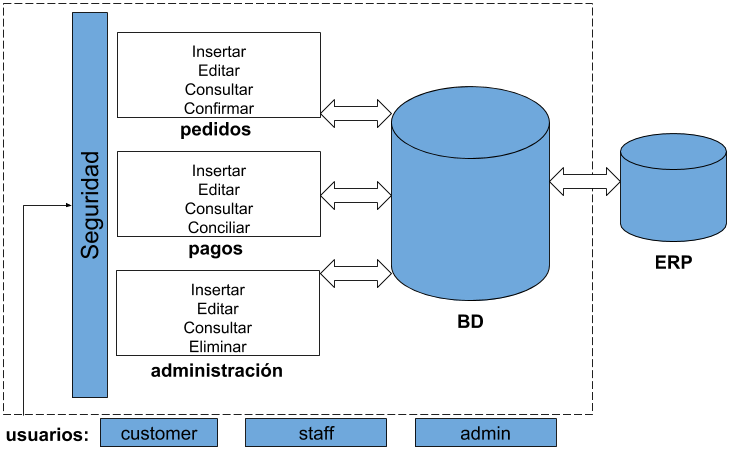
\includegraphics[width=\textwidth]{esquema_general_nuevo.png}
    \caption{Esquema general de los módulos de funcionalidad}
    \label{fig:esquema_general_nuevo}
    \centering
\end{figure}

Uno de los objetivos de la aplicación es servir como sistema de apoyo a los ERP de los mayoristas. Los sistemas ERP llevan el control de todas las entidades del negocio, entre estas están las estaciones de servicio, los transportes para los pedidos, los pedidos, las facturas, etc. La aplicación eFuel interactúa con el sistema ERP y le sirve de apoyo a este manteniendo un registro separado de las entidades pertinentes a la inserción y el pago de pedidos de combustible. Esta interacción se da a través de importaciones y exportaciones de datos entre estos sistemas para que estén sincronizados. En la figura \ref{fig:domain_model} se describe esta interacción con el sistema ERP.

\section{Fases del desarrollo}
\subsection{Fase de Inducción}
Esta fase tuvo una duración de 1 semana, el pasante realizó varios tutoriales y utilizó varios recursos (guías de Umbraco, videos de ASP.NET, entre otros) proporcionados por la empresa para inducir los conocimientos técnicos necesarios para llevar a cabo el proyecto. Las herramientas investigadas fueron: Umbraco, ASP.NET, SQL Server y Visual Studio.

Aunque esta fase estuvo exclusivamente dedicada al aprendizaje hay que remarcar que, durante toda la pasantía, el pasante adquirió nuevas destrezas que fueron necesarias y facilitaron el desarrollo del proyecto. Una vez culminada esta fase se empezó el desarrollo de la aplicación.


\subsection{Fase de Desarrollo}
Esta fase duró 16 semanas continuas y se llevaron a cabo 6 Iteraciones donde se desarrolló la aplicación. A continuación una descripción del trabajo realizado en cada iteración.

\subsubsection{Análisis de requerimientos (1era Iteración)}
Se definió el alcance inicial del proyecto, la arquitectura y la estructura de la base de datos. Además, se creó el repositorio de Git, el proyecto de Visual Studio y el sitio de Umbraco, y por otro lado, se eligió una plantilla de HTML para el \emph{look and feel} de la aplicación.

\textbf{Actividades realizadas:}
\begin{itemize}
    \item Familiarización con la versión original de eFuel.
    \item Definir las reglas de negocio para el sistema.
    \item Definir los actores del sistema.
    \item Se listaron las funcionalidades básicas a desarrollar.
    \item Creación de la solución de Visual Studio.
    \item Creación del repositorio de Git y familiarización con las reglas del mismo.
    \item Se definieron las entidades de la base de datos del proyecto para poder implementar funcionalidades básicas del sistema.
    \item Se creó el sitio de Umbraco.
    \item Se evaluaron las plantillas para el front end de la aplicación y se eligió una.
\end{itemize}

\textbf{Duración:} 2 semanas.

\subsubsection{Módulo de Administración (2da Iteración)}
Se implementó la funcionalidad de manejo de las entidades principales de la aplicación: clientes, productos, transportes, zonas, turnos, pedidos, facturas y cobros. Para esto se implementó una interfaz en el back end de Umbraco usando Fluidity y se definieron los Doctypes y Datatypes de las entidades a ser almacenadas como contenido de Umbraco. También se empezó el desarrollo del front end de la aplicación. Al finalizar esta Iteración se tuvo una forma de manejar las entidades del sistema, ya sea a través del árbol de contenido de Umbraco o a través de la interfaz de Fluidity.

\textbf{Actividades realizadas:}
\begin{itemize}
    \item Se definieron los Doctypes y Datatypes para las entidades que serán manejadas a través de Umbraco.
    \item Se desarrolló la interfaz de Fluidity para insertar registros en la base de datos de las entidades que serán manejadas directamente con esta.
    \item Se empezó el desarrollo del front end de la aplicación, esto es, de los elementos en común que tendrán todas las páginas: navbar, título, etc.
    \item Se desarrollaron las vistas de listado de facturas, transportes y zonas en el front end.
\end{itemize}

\textbf{Duración:} 3 semanas.

\subsubsection{Módulo de Pedidos (3ra Iteración)}
Esta Iteración estuvo dedicada al desarrollo de la funcionalidad referente a los pedidos de combustible. Se desarrolló el listado de pedido con filtros, el formulario de creación de pedidos y la exportación de la lista de pedidos.

\textbf{Actividades realizadas:}
\begin{itemize}
    \item Desarrollo de la vista de listado de pedidos.
    \item Implementación de los filtros para la lista de pedidos.
    \item Implementación de la vista de detalles de un pedido.
    \item Mejoras al código y funcionalidad desarrolladas en las demás Iteraciones.
\end{itemize}

\textbf{Duración:} 2 semanas.

\subsubsection{Refactorización (4ta Iteración)}
En esta Iteración se determinó que la implementación de la funcionalidad desarrollada hasta ahora no estaba siguiendo la estructura de la solución de Visual Studio, es decir, los controladores no estaban bien organizados según el patrón MVC (como lo implementa ASP.NET) y que además había funcionalidad que debería estar implementada en \verb|EF_API| pero que estaba en \verb|EF_Core| y usando el tipo de controlador incorrecto. Esto se debió a un a falta de comunicación entre el dueño del producto y el pasante. Se realizaron las correcciones necesarias, esto tomó tiempo que no pudo ser invertido en el desarrollo de unos de los módulos planteados en el plan de trabajo original (Módulo de conciliación de pagos), en consecuencia, los casos de uso de este módulo quedaron parcialmente implementados.

\textbf{Actividades realizadas:}
\begin{itemize}
    \item Reorganización de los controladores de la aplicación.
    \item Refactorización del código en gran parte de la funcionalidad.
    \item Mejoras en la calidad del código.
\end{itemize}

\textbf{Duración:} 3 semanas.

\subsubsection{Continuación con el Módulo de Pedidos (5ta Iteración)}
En esta Iteración se continuó el desarrollo de la funcionalidad referente a los pedidos del sistema y se mejoraron algunos aspectos implementados en las otras Iteraciones.

\textbf{Actividades realizadas:}
\begin{itemize}
    \item Implementación del formulario de crear pedido.
    \item Implementación de la exportación de la lista de pedidos.
    \item Mejoras generales en el código de la aplicación.
\end{itemize}

\textbf{Duración:} 3 semanas.

\subsubsection{Módulo de Manejo de Usuarios e importación (6ta Iteración)}
Esta fue la última Iteración de desarrollo, en ella se desarrollo el módulo de manejo de usuarios y se implementó la funcionalidad de importación de algunas entidades. También se mejoraron todos los aspectos que fueron posibles del código.

\textbf{Actividades realizadas:}
\begin{itemize}
    \item Se definieron los miembros (Members de Umbraco) y los permisos por actor (customer y staff).
    \item Implementación de autenticación, inicio y cierre de sesión para el front end de la aplicación.
    \item Implementación de importación de Zonas y Transportes.
    \item Elaboración de la guía de instalación de la aplicación (ver anexo \ref{installationGuide}).
    \item Mejoras del código y corrección de bugs.
\end{itemize}

\textbf{Duración:} 3 semanas.

\subsection{Fase de Documentación} \label{documentation}
Esta fase duró el resto de las 20 semanas totales de la pasantía. En ella se documentó el estado final de la aplicación, se elaboró un Documento de Arquitectura de Software donde se detallan los componentes y casos de uso desarrollados de la aplicación y, además, se elaboró una guía de instalación de eFuel (ver apéndice \ref{installationGuide}). En total esto llevo 3 semanas de la pasantía y algunas extra después de culminada.

\subsubsection{Arquitectura del sistema}
A continuación se muestran el Modelo de Dominio y el Diagrama de Componentes del sistema que ayudan a describir la arquitectura del mismo y que fueron parte del trabajo realizado durante la fase de documentación (ver sección \ref{documentation}). El Modelo de Dominio ayuda a entender la relación de eFuel con el sistema ERP del mayorista. Por otro lado, el Diagrama de Componentes refleja como fue utilizado el patrón MVC en la arquitectura del sistema. Para una decripción detallada de la arquitectura del sistema referirse al anexo \ref{das}, donde se encuentra el Documento de Arquitectura de Software de eFuel.

\begin{figure}[H]
    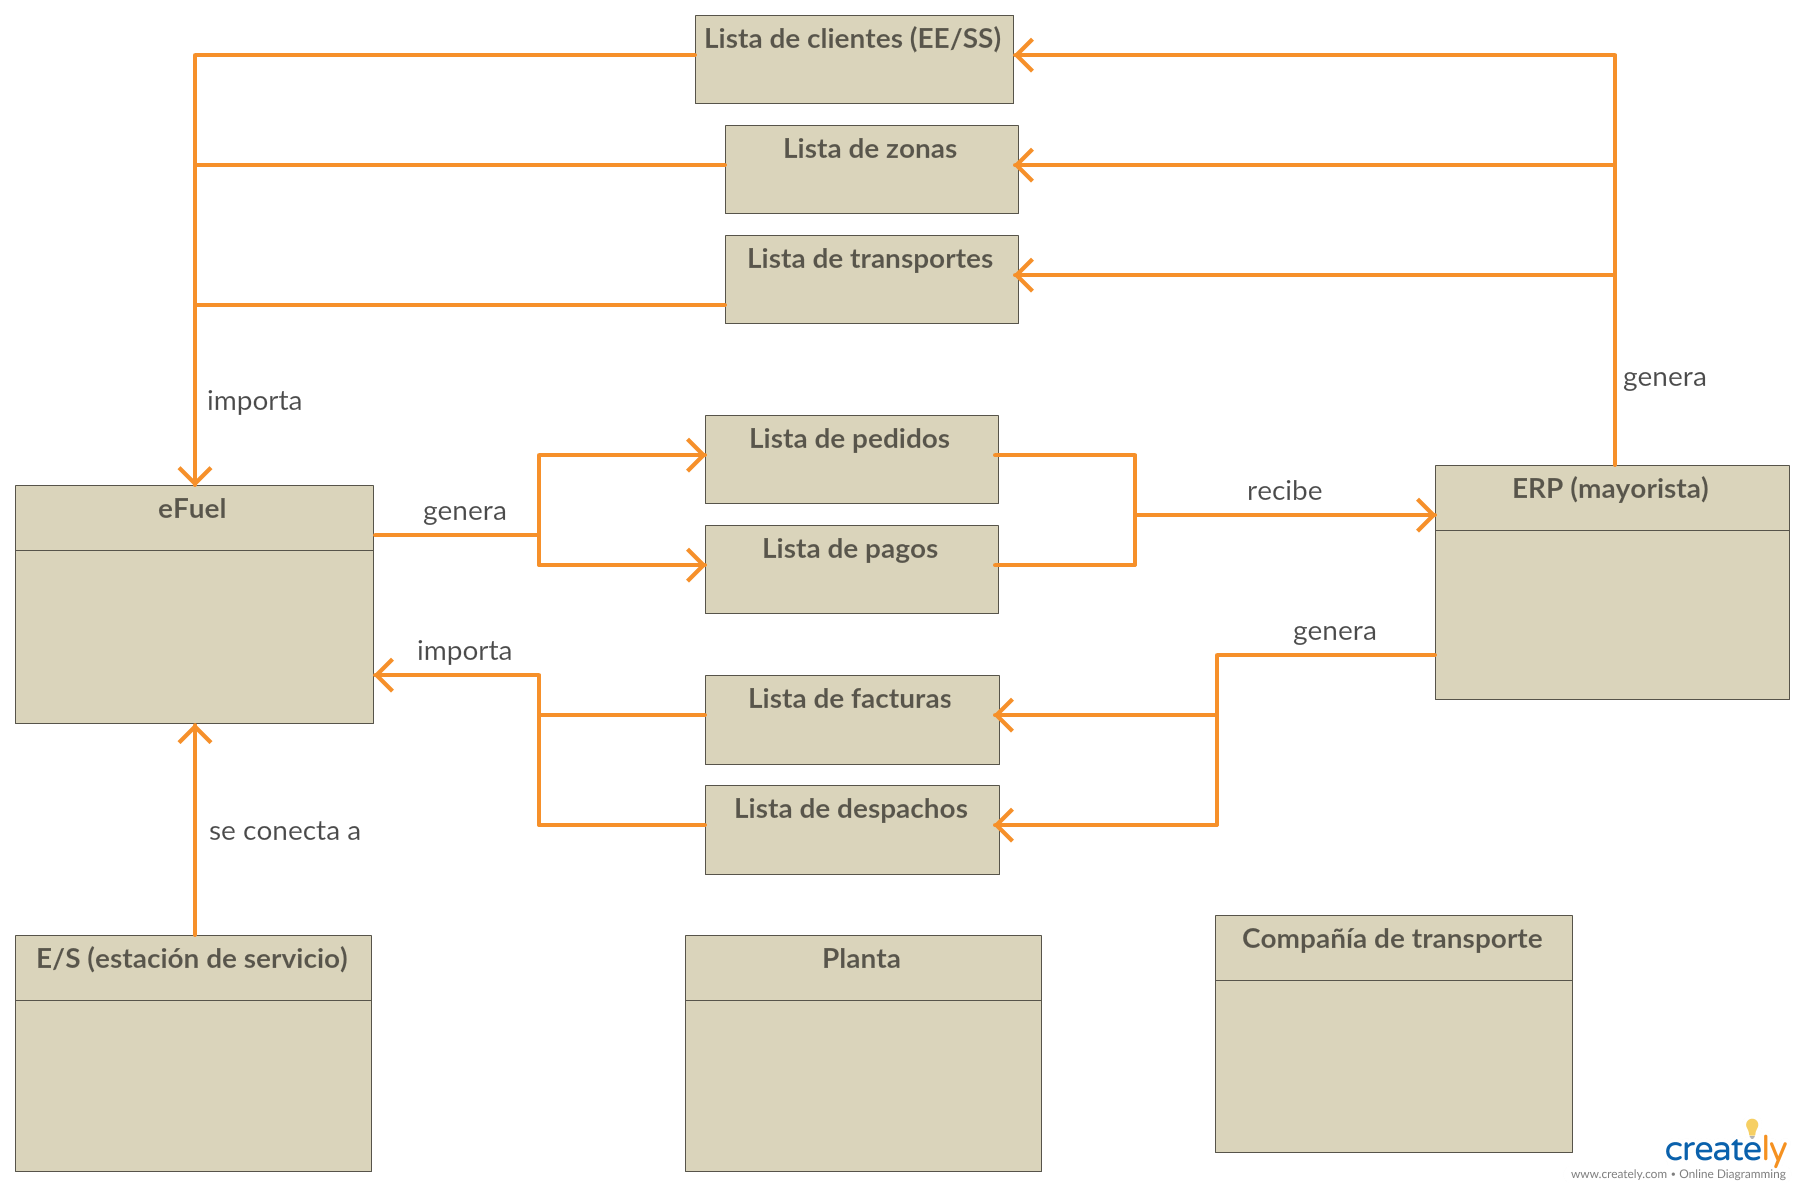
\includegraphics[width=\textwidth]{domain_model.png}
    \caption{Modelo de dominio de eFuel}
    \label{fig:domain_model}
    \centering
\end{figure}

\begin{figure}[H]
    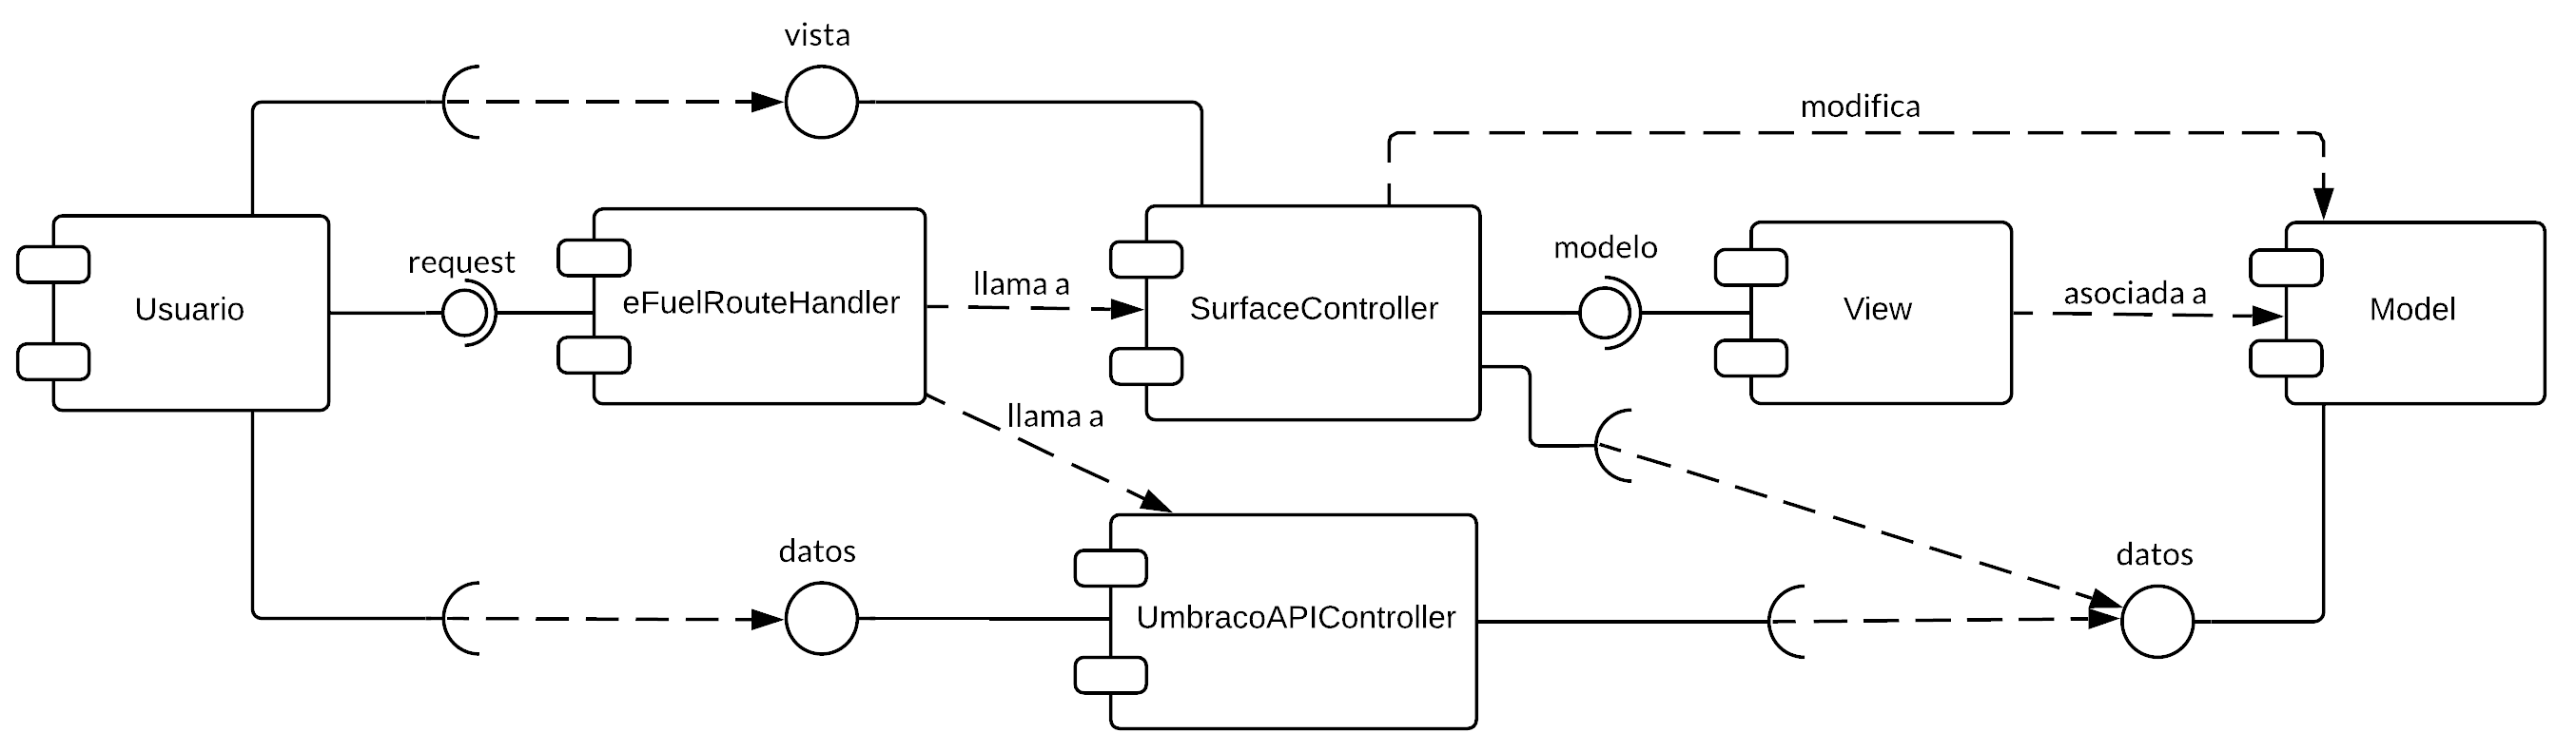
\includegraphics[width=\textwidth]{component_diagram.png}
    \caption{Diagrama de Componentes de eFuel}
    \label{fig:component_diagram}
    \centering
\end{figure}